\documentclass[a4paper,11pt]{article}\usepackage[]{graphicx}\usepackage[]{color}
%% maxwidth is the original width if it is less than linewidth
%% otherwise use linewidth (to make sure the graphics do not exceed the margin)
\makeatletter
\def\maxwidth{ %
  \ifdim\Gin@nat@width>\linewidth
    \linewidth
  \else
    \Gin@nat@width
  \fi
}
\makeatother

\definecolor{fgcolor}{rgb}{0.345, 0.345, 0.345}
\newcommand{\hlnum}[1]{\textcolor[rgb]{0.686,0.059,0.569}{#1}}%
\newcommand{\hlstr}[1]{\textcolor[rgb]{0.192,0.494,0.8}{#1}}%
\newcommand{\hlcom}[1]{\textcolor[rgb]{0.678,0.584,0.686}{\textit{#1}}}%
\newcommand{\hlopt}[1]{\textcolor[rgb]{0,0,0}{#1}}%
\newcommand{\hlstd}[1]{\textcolor[rgb]{0.345,0.345,0.345}{#1}}%
\newcommand{\hlkwa}[1]{\textcolor[rgb]{0.161,0.373,0.58}{\textbf{#1}}}%
\newcommand{\hlkwb}[1]{\textcolor[rgb]{0.69,0.353,0.396}{#1}}%
\newcommand{\hlkwc}[1]{\textcolor[rgb]{0.333,0.667,0.333}{#1}}%
\newcommand{\hlkwd}[1]{\textcolor[rgb]{0.737,0.353,0.396}{\textbf{#1}}}%
\let\hlipl\hlkwb

\usepackage{framed}
\makeatletter
\newenvironment{kframe}{%
 \def\at@end@of@kframe{}%
 \ifinner\ifhmode%
  \def\at@end@of@kframe{\end{minipage}}%
  \begin{minipage}{\columnwidth}%
 \fi\fi%
 \def\FrameCommand##1{\hskip\@totalleftmargin \hskip-\fboxsep
 \colorbox{shadecolor}{##1}\hskip-\fboxsep
     % There is no \\@totalrightmargin, so:
     \hskip-\linewidth \hskip-\@totalleftmargin \hskip\columnwidth}%
 \MakeFramed {\advance\hsize-\width
   \@totalleftmargin\z@ \linewidth\hsize
   \@setminipage}}%
 {\par\unskip\endMakeFramed%
 \at@end@of@kframe}
\makeatother

\definecolor{shadecolor}{rgb}{.97, .97, .97}
\definecolor{messagecolor}{rgb}{0, 0, 0}
\definecolor{warningcolor}{rgb}{1, 0, 1}
\definecolor{errorcolor}{rgb}{1, 0, 0}
\newenvironment{knitrout}{}{} % an empty environment to be redefined in TeX

\usepackage{alltt}

\usepackage[left=2.5cm,right=2.5cm,top=3cm,bottom=3cm,pdftex]{geometry}
\usepackage{amssymb, amsmath, url, natbib, float, subcaption, listings,mathtools}
\usepackage[utf8]{inputenc}
\usepackage[T1]{fontenc}
\usepackage[pdftex]{graphicx}

\DeclareGraphicsExtensions{.png, .pdf, .jpg}
\usepackage[pdftex, colorlinks, linkcolor=blue, urlcolor=blue, citecolor=blue, pagecolor=blue, breaklinks=true]{hyperref}
\IfFileExists{upquote.sty}{\usepackage{upquote}}{}
\begin{document}

\pagestyle{empty}
\title{Comparison}
\begin{center}
\Large\textbf{CRAN packages comparison} \\[11pt]
\normalsize
\end{center}

\section{DiffusionRgqd}
Uses the cumulant truncation procedure developed by Varughese (2013), whereby the transition density can be approximated over arbitrarily large transition horizons for a suitably general class of non-linear diffusion models.

Generalized quadratic diffusions (GQD) are the specific class of SDEs with quadratic drift and diffusion terms:

\begin{align*}
d X_t & = \mu(X_t, t)dt + \sigma(X_t, t)dW_t, \: \text{where} \\
\mu(X_t, t) & = G_0(t) + G_1(t) X_t + G_2(t) X_t^2, \: \text{and} \\
\sigma (X_t, t) & = Q_0(t) + Q_1(t) X_t + Q_2(t) X_t^2
\end{align*}

For purposes of inference the drift and diffusion terms - and consequently the transitional density - are assumed to be dependent on a vector of parameters, $\theta$. For example, an Ornstein-Uhlenbeck model with SDE:

\begin{equation}
d X_t = \theta_1 (\theta_2 - X_t) + \sqrt{\theta_3^2} dW_t
\end{equation}

\begin{knitrout}
\definecolor{shadecolor}{rgb}{0.969, 0.969, 0.969}\color{fgcolor}\begin{kframe}
\begin{alltt}
\hlstd{G0}\hlkwb{=}\hlkwa{function}\hlstd{(}\hlkwc{t}\hlstd{)\{theta[}\hlnum{1}\hlstd{]}\hlopt{*}\hlstd{theta[}\hlnum{2}\hlstd{]\}}
\hlstd{G1}\hlkwb{=}\hlkwa{function}\hlstd{(}\hlkwc{t}\hlstd{)\{}\hlopt{-}\hlstd{theta[}\hlnum{1}\hlstd{]\}}
\hlstd{Q0}\hlkwb{=}\hlkwa{function}\hlstd{(}\hlkwc{t}\hlstd{)\{theta[}\hlnum{3}\hlstd{]}\hlopt{*}\hlstd{theta[}\hlnum{3}\hlstd{]\}}
\end{alltt}
\end{kframe}
\end{knitrout}

\subsection{Constant drift, diffusion SDE}
For a constant drift, diffusion SDE, with given initial condition $X_s$:
\begin{equation}
dX_t = \mu dt + \sigma dW_t
\end{equation}
The distribution at time $t$ of the process $X_t$ is $\mathcal{N}(X_t, X_s + \mu(t-s), \sigma^2(t-s))$

\begin{knitrout}
\definecolor{shadecolor}{rgb}{0.969, 0.969, 0.969}\color{fgcolor}\begin{kframe}
\begin{alltt}
\hlkwd{library}\hlstd{(}\hlstr{'DiffusionRgqd'}\hlstd{)}

\hlcom{# Remove any existing coefficients}
\hlkwd{GQD.remove}\hlstd{()}

\hlstd{Xs} \hlkwb{<-} \hlnum{0}                 \hlcom{# Initial state}
\hlstd{Xt} \hlkwb{<-} \hlkwd{seq}\hlstd{(}\hlopt{-}\hlnum{3}\hlopt{/}\hlnum{2}\hlstd{,}\hlnum{3}\hlopt{/}\hlnum{2}\hlstd{,}\hlnum{1}\hlopt{/}\hlnum{50}\hlstd{)}\hlcom{# Possible future states}
\hlstd{s}  \hlkwb{<-} \hlnum{0}                 \hlcom{# Starting time}
\hlstd{t}  \hlkwb{<-} \hlnum{1}                 \hlcom{# Final time}
\hlstd{mu}    \hlkwb{<-} \hlnum{0.5}            \hlcom{# Drift parameter}
\hlstd{sigma} \hlkwb{<-} \hlnum{0.25}           \hlcom{# Diffusion coefficient}

\hlcom{# Define the model coefficients}
\hlstd{G0} \hlkwb{<-} \hlkwa{function}\hlstd{(}\hlkwc{t}\hlstd{)\{mu\}}
\hlstd{Q0} \hlkwb{<-} \hlkwa{function}\hlstd{(}\hlkwc{t}\hlstd{)\{sigma}\hlopt{^}\hlnum{2}\hlstd{\}}

\hlcom{# Calculate the transitional density}
\hlstd{BM} \hlkwb{<-} \hlkwd{GQD.density}\hlstd{(Xs,Xt,s,t)}

\hlcom{# Plot the transitional density}
\hlkwd{plot}\hlstd{(}\hlkwd{dnorm}\hlstd{(Xt, Xs}\hlopt{+}\hlstd{mu}\hlopt{*}\hlstd{(t}\hlopt{-}\hlstd{s), sigma}\hlopt{*}\hlkwd{sqrt}\hlstd{(t}\hlopt{-}\hlstd{s))}\hlopt{~}\hlstd{Xt,} \hlkwc{main} \hlstd{=} \hlstr{'Transition density'}\hlstd{,} \hlkwc{type} \hlstd{=} \hlstr{'l'}\hlstd{)}
\hlkwd{lines}\hlstd{(BM}\hlopt{$}\hlstd{density[,}\hlnum{100}\hlstd{]}\hlopt{~}\hlstd{BM}\hlopt{$}\hlstd{Xt,} \hlkwc{col} \hlstd{=} \hlstr{'blue'}\hlstd{,} \hlkwc{lty} \hlstd{=} \hlstr{'dashed'}\hlstd{,} \hlkwc{lwd} \hlstd{=} \hlnum{2}\hlstd{)}
\end{alltt}
\end{kframe}
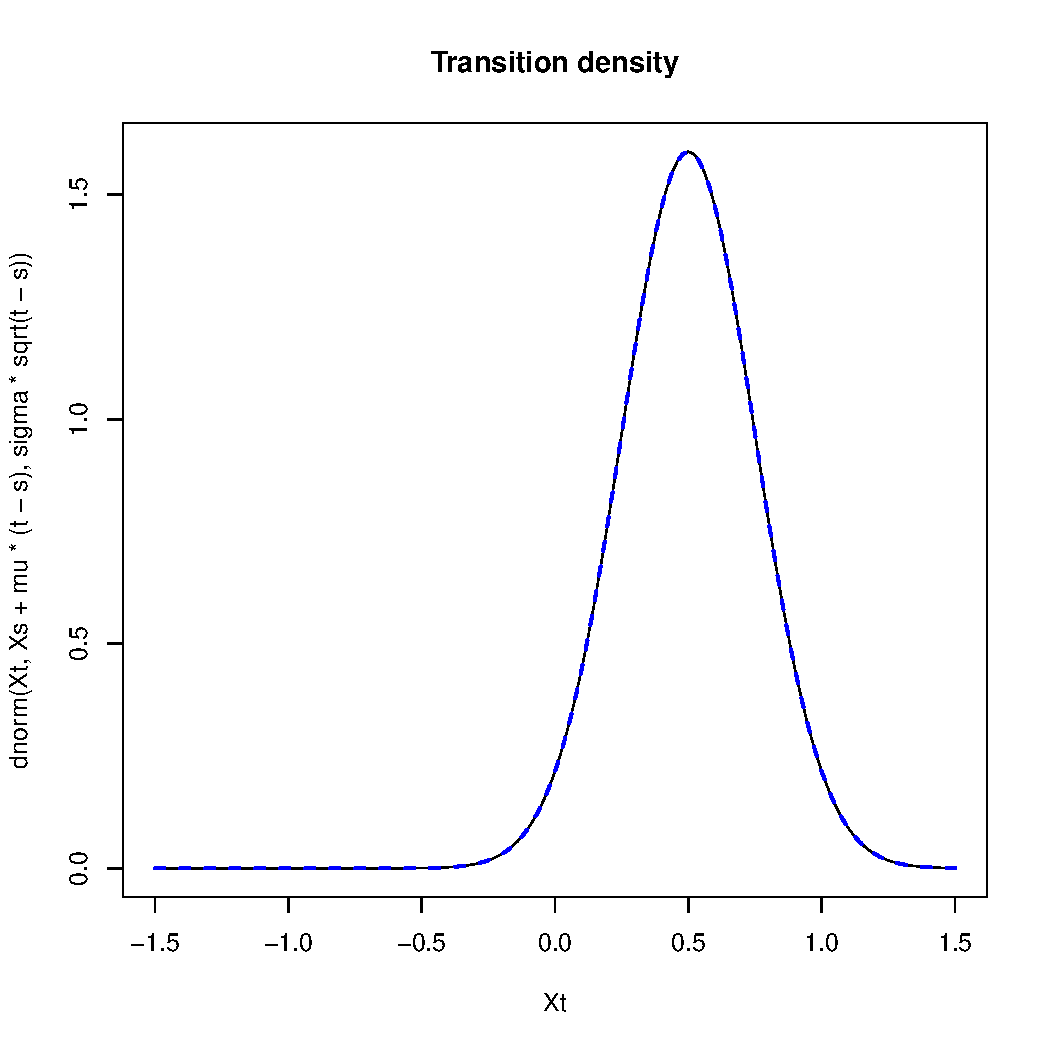
\includegraphics[width=4in,height=4in]{figure/GQD-brownian-1} 

\end{knitrout}

\subsection{CIR process}
Another example using the CIR process SDE:
\begin{equation}
dX_t = \theta_1 (\theta_2 - X_t)dt + \theta_3 \sqrt{X_t} dW_t
\end{equation}

\begin{knitrout}
\definecolor{shadecolor}{rgb}{0.969, 0.969, 0.969}\color{fgcolor}\begin{kframe}
\begin{alltt}
\hlkwd{GQD.remove}\hlstd{()}
\hlstd{a} \hlkwb{=} \hlnum{0.5}\hlstd{; b} \hlkwb{=} \hlnum{5}\hlstd{; sigma} \hlkwb{=} \hlnum{0.35}\hlstd{;} \hlcom{# Parameter values}

\hlstd{G0} \hlkwb{<-} \hlkwa{function}\hlstd{(}\hlkwc{t}\hlstd{)\{a}\hlopt{*}\hlstd{b\}}
\hlstd{G1} \hlkwb{<-} \hlkwa{function}\hlstd{(}\hlkwc{t}\hlstd{)\{}\hlopt{-}\hlstd{a\}}
\hlstd{Q1} \hlkwb{<-} \hlkwa{function}\hlstd{(}\hlkwc{t}\hlstd{)\{sigma}\hlopt{^}\hlnum{2}\hlstd{\}}

\hlstd{states}     \hlkwb{<-}  \hlkwd{seq}\hlstd{(}\hlnum{1}\hlstd{,} \hlnum{9}\hlstd{,} \hlnum{1}\hlopt{/}\hlnum{10}\hlstd{)}\hlcom{# State values}
\hlstd{initial}    \hlkwb{<-}  \hlnum{6}              \hlcom{# Starting value of the process}
\hlstd{Tmax}       \hlkwb{<-}  \hlnum{5}              \hlcom{# Time horizon}
\hlstd{Tstart}     \hlkwb{<-}  \hlnum{1}              \hlcom{# Time starts at 1}
\hlstd{increment}  \hlkwb{<-}  \hlnum{1}\hlopt{/}\hlnum{100}          \hlcom{# Incremental time steps}

\hlcom{# Generate the transitional density}
\hlstd{M} \hlkwb{<-} \hlkwd{GQD.density}\hlstd{(}\hlkwc{Xs} \hlstd{= initial,} \hlkwc{Xt} \hlstd{= states,} \hlkwc{s} \hlstd{= Tstart,} \hlkwc{t} \hlstd{= Tmax,} \hlkwc{delt} \hlstd{= increment)}

\hlkwd{persp}\hlstd{(}\hlkwc{x} \hlstd{= M}\hlopt{$}\hlstd{Xt,} \hlkwc{y} \hlstd{= M}\hlopt{$}\hlstd{time,} \hlkwc{z} \hlstd{= M}\hlopt{$}\hlstd{density,} \hlkwc{col} \hlstd{=} \hlstr{'white'}\hlstd{,} \hlkwc{xlab} \hlstd{=} \hlstr{'State (X_t)'}\hlstd{,}\hlkwc{ylab}
 \hlstd{=} \hlstr{'Time (t)'}\hlstd{,} \hlkwc{zlab} \hlstd{=} \hlstr{'Density f(X_t|X_s)'}\hlstd{,} \hlkwc{border} \hlstd{=} \hlnum{NA}\hlstd{,} \hlkwc{shade} \hlstd{=} \hlnum{0.5}\hlstd{,} \hlkwc{theta} \hlstd{=} \hlnum{145}\hlstd{)}
\end{alltt}
\end{kframe}
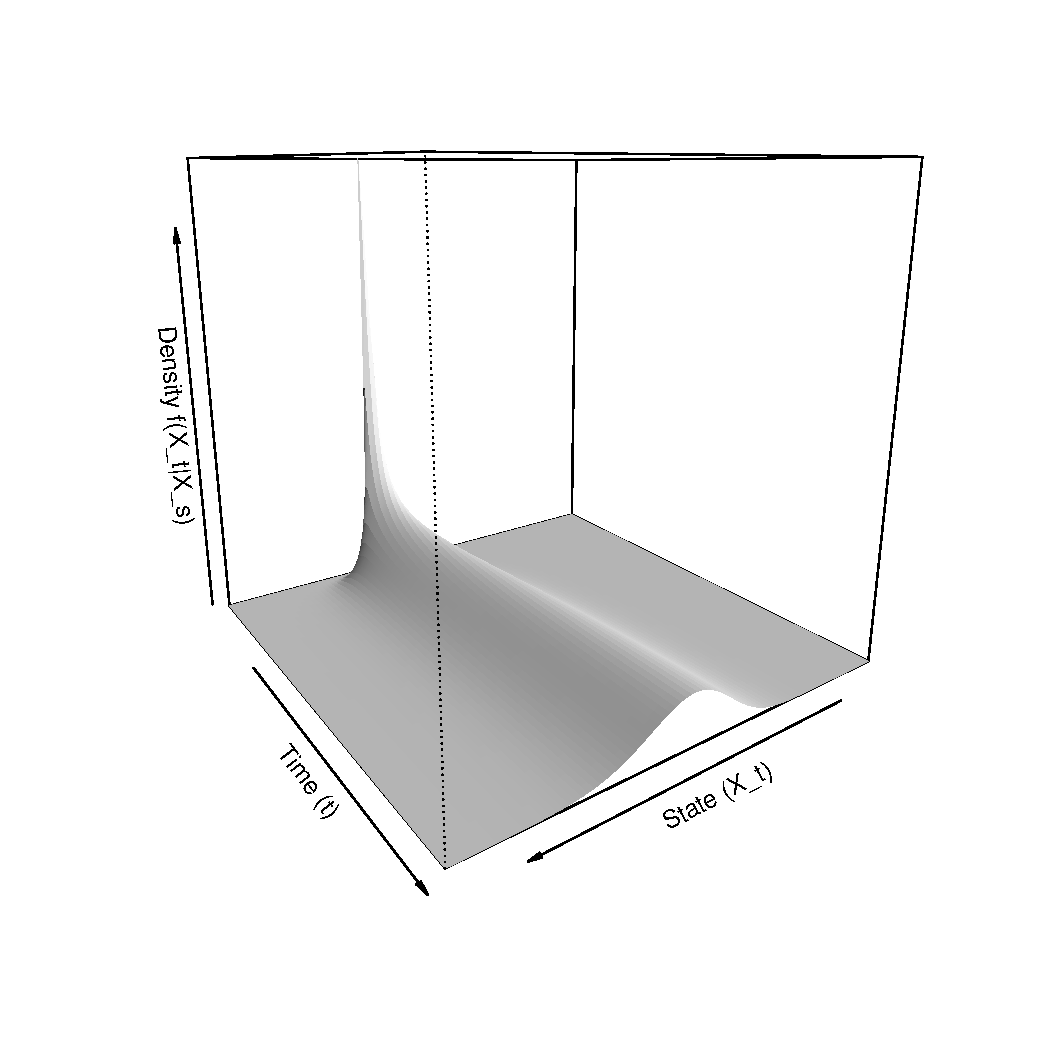
\includegraphics[width=4in,height=4in]{figure/GQD-CIR-1} 

\end{knitrout}

The GQD.density() returns (density, Xt, time, cumulants, moments, mesh). 

%The progression of mean and variance follows:
%<<GQD-meanvar, out.width='4in', out.height='4in'>>=
%plot(M$cumulants[1,]~M$time, main = 'Mean trajectory', type = 'l')
%plot(M$cumulants[2,]~M$time, main = 'Variance trajectory', type  = 'l')
%@

\subsection{Time dependent CIR process}
Consider the time-inhomogeneous CIR process for a more complicated example

\begin{equation}
dX_t = 2(10 + \sin(2 \pi (t - 0.5)) - X_t) dt + sqrt{0.25 (1 + 0.75 \sin(4 \pi t))X_t} dW_t
\end{equation}

\begin{knitrout}
\definecolor{shadecolor}{rgb}{0.969, 0.969, 0.969}\color{fgcolor}\begin{kframe}
\begin{alltt}
\hlkwd{library}\hlstd{(DiffusionRgqd)}
\hlkwd{GQD.remove}\hlstd{()}
\hlstd{G0} \hlkwb{<-} \hlkwa{function}\hlstd{(}\hlkwc{t}\hlstd{)\{}\hlnum{2}\hlopt{*}\hlstd{(}\hlnum{10}\hlopt{+}\hlkwd{sin}\hlstd{(}\hlnum{2}\hlopt{*}\hlstd{pi}\hlopt{*}\hlstd{(t}\hlopt{-}\hlnum{0.5}\hlstd{)))\}}
\hlstd{G1} \hlkwb{<-} \hlkwa{function}\hlstd{(}\hlkwc{t}\hlstd{)\{}\hlopt{-}\hlnum{2}\hlstd{\}}
\hlstd{Q1} \hlkwb{<-} \hlkwa{function}\hlstd{(}\hlkwc{t}\hlstd{)\{}\hlnum{0.25}\hlopt{*}\hlstd{(}\hlnum{1}\hlopt{+}\hlnum{0.75}\hlopt{*}\hlstd{(}\hlkwd{sin}\hlstd{(}\hlnum{4}\hlopt{*}\hlstd{pi}\hlopt{*}\hlstd{t)))\}}

\hlstd{states}    \hlkwb{<-} \hlkwd{seq}\hlstd{(}\hlnum{5}\hlstd{,} \hlnum{15}\hlstd{,} \hlnum{1}\hlopt{/}\hlnum{10}\hlstd{)}
\hlstd{initial}   \hlkwb{<-} \hlnum{8}
\hlstd{Tmax}      \hlkwb{<-} \hlnum{5}
\hlstd{Tstart}    \hlkwb{<-} \hlnum{1}
\hlstd{increment} \hlkwb{<-} \hlnum{1}\hlopt{/}\hlnum{100}

\hlstd{M} \hlkwb{<-} \hlkwd{GQD.density}\hlstd{(}\hlkwc{Xs} \hlstd{= initial,} \hlkwc{Xt} \hlstd{= states,} \hlkwc{s} \hlstd{= Tstart,} \hlkwc{t} \hlstd{= Tmax,} \hlkwc{delt} \hlstd{= increment)}
\hlkwd{persp}\hlstd{(}\hlkwc{x} \hlstd{= M}\hlopt{$}\hlstd{Xt,} \hlkwc{y} \hlstd{= M}\hlopt{$}\hlstd{time,} \hlkwc{z} \hlstd{= M}\hlopt{$}\hlstd{density,} \hlkwc{col} \hlstd{=} \hlstr{'white'}\hlstd{,} \hlkwc{xlab} \hlstd{=} \hlstr{'State (X_t)'}\hlstd{,} \hlkwc{ylab} \hlstd{=} \hlstr{'Time (t)'}\hlstd{,} \hlkwc{zlab} \hlstd{=} \hlstr{'Density f(X_t|X_s)'}\hlstd{,} \hlkwc{border} \hlstd{=} \hlnum{NA}\hlstd{,} \hlkwc{shade} \hlstd{=} \hlnum{0.5}\hlstd{,} \hlkwc{theta} \hlstd{=} \hlnum{145}\hlstd{)}
\end{alltt}
\end{kframe}
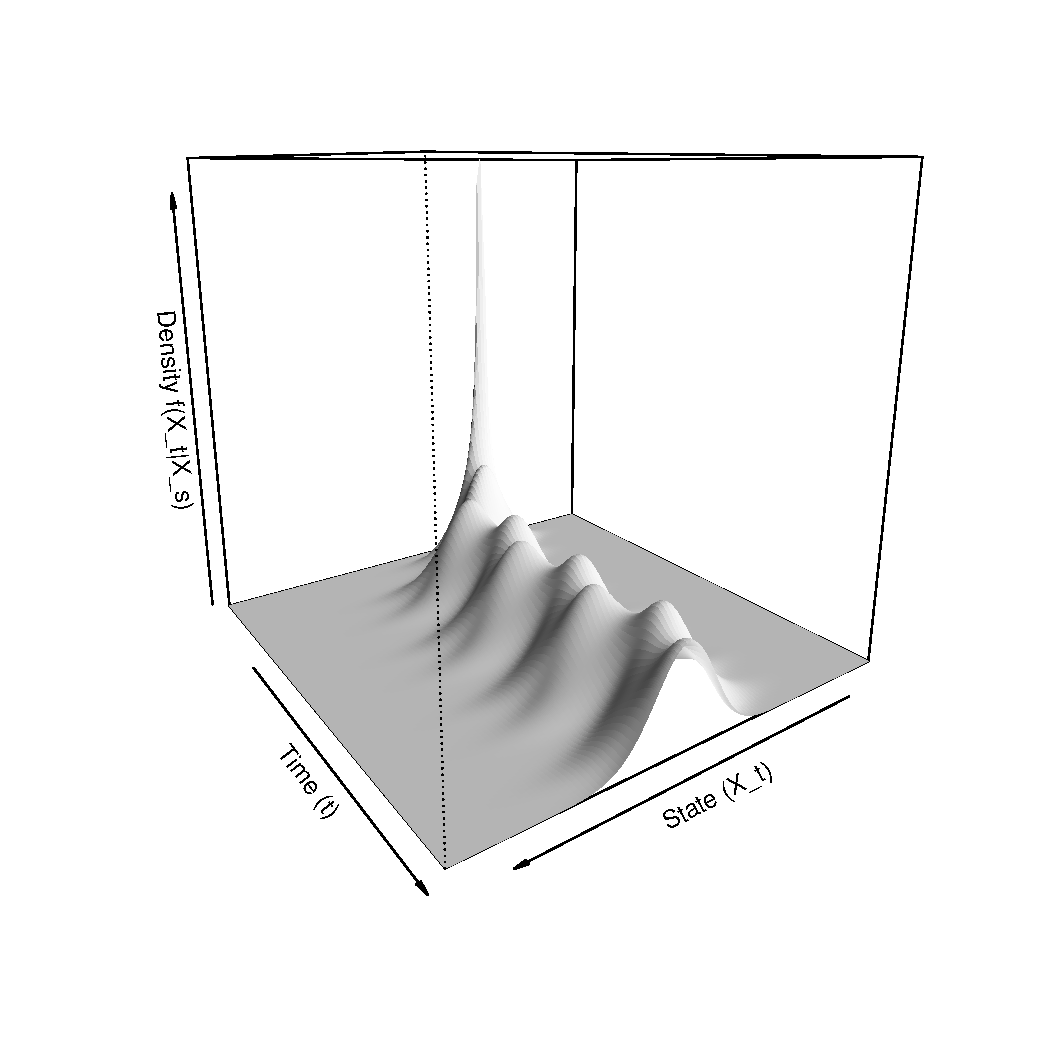
\includegraphics[width=4in,height=4in]{figure/GQD-tCIR-1} 

\end{knitrout}

\subsection{Coupled SDEs - Prey predator model}
A model that is often used to illustrate non-linear dynamics in the analysis of ODEs is that of the Lotka-Volterra model. The equations are often used to describe the dynamics of two interacting populations wherein the population growth rate of the populations are mutually influenced by the current level of the opposing population. As such the model has been used to explain oscillatory behaviour in predator-prey relationships {Hoppensteadt2006} where xtxt denotes the prey population and ytyt the predator population at time $t$. Continuing with the predator-prey metaphor, perhaps one deficiency of the model, one might argue, is the absence of random input and subsequent effects on population levels. Indeed, under the ODE formulation the predicted population behaviour (given fixed parameters) are completely deterministic. Another deficiency might be the absence of growth inhibiting factors such as disease or over-grazing. For these purposes we may define an example of a stochastic counterpart to the Lotka-Volterra equations as:

\begin{align*}
dX_t & = (aX_t - bX_t Y_t) dt + f \sqrt{X_t} dW^1_t \\
dY_t & = (-cY_t + dX_t Y_t - eY^2_t)dt + g \sqrt{Y_t} dW^2_t
\end{align*}

\begin{knitrout}
\definecolor{shadecolor}{rgb}{0.969, 0.969, 0.969}\color{fgcolor}\begin{kframe}
\begin{alltt}
\hlkwd{library}\hlstd{(DiffusionRgqd)}
\hlcom{# Remove any existing coefficients:}
\hlkwd{GQD.remove}\hlstd{()}
\end{alltt}
\begin{verbatim}
## [1] "Removed :  G0 G1 Q1"
\end{verbatim}
\begin{alltt}
\hlcom{# Define the X dimesnion coefficients:}
\hlstd{a10} \hlkwb{<-} \hlkwa{function}\hlstd{(}\hlkwc{t}\hlstd{)\{}\hlnum{1.5}\hlstd{\}}
\hlstd{a11} \hlkwb{<-} \hlkwa{function}\hlstd{(}\hlkwc{t}\hlstd{)\{}\hlopt{-}\hlnum{0.4}\hlstd{\}}
\hlstd{c10} \hlkwb{<-} \hlkwa{function}\hlstd{(}\hlkwc{t}\hlstd{)\{}\hlnum{0.05}\hlstd{\}}
\hlcom{# Define the Y dimension coefficients:}
\hlstd{b01} \hlkwb{<-} \hlkwa{function}\hlstd{(}\hlkwc{t}\hlstd{)\{}\hlopt{-}\hlnum{1.5}\hlstd{\}}
\hlstd{b11} \hlkwb{<-} \hlkwa{function}\hlstd{(}\hlkwc{t}\hlstd{)\{}\hlnum{0.4}\hlstd{\}}
\hlstd{b02} \hlkwb{<-} \hlkwa{function}\hlstd{(}\hlkwc{t}\hlstd{)\{}\hlopt{-}\hlnum{0.2}\hlstd{\}}
\hlstd{f01} \hlkwb{<-} \hlkwa{function}\hlstd{(}\hlkwc{t}\hlstd{)\{}\hlnum{0.1}\hlstd{\}}
\hlcom{# Approximate the transition density}
\hlstd{res} \hlkwb{<-} \hlkwd{BiGQD.density}\hlstd{(}\hlkwc{Xs} \hlstd{=} \hlnum{5}\hlstd{,} \hlkwc{Ys} \hlstd{=} \hlnum{5}\hlstd{,} \hlkwc{Xt} \hlstd{=} \hlkwd{seq}\hlstd{(}\hlnum{3}\hlstd{,} \hlnum{8}\hlstd{,} \hlkwc{length} \hlstd{=} \hlnum{50}\hlstd{),} \hlkwc{Yt} \hlstd{=} \hlkwd{seq}\hlstd{(}\hlnum{2}\hlstd{,} \hlnum{6}\hlstd{,} \hlkwc{length} \hlstd{=} \hlnum{50}\hlstd{),} \hlkwc{s} \hlstd{=} \hlnum{0}\hlstd{,} \hlkwc{t} \hlstd{=} \hlnum{10}\hlstd{,} \hlkwc{delt} \hlstd{=} \hlnum{1}\hlopt{/}\hlnum{100}\hlstd{)}
\end{alltt}
\begin{verbatim}
##                                                                  
##  ================================================================
##                    GENERALIZED QUADRATIC DIFFUSON                
##  ================================================================
##  _____________________ Drift Coefficients _______________________
##  a10 : 1.5                                                       
##  a11 : -0.4                                                      
##  ...   ...   ...   ...   ...   ...   ...   ...   ...   ...   ... 
##  b01 : -1.5                                                      
##  b02 : -0.2                                                      
##  b11 : 0.4                                                       
##  ___________________ Diffusion Coefficients _____________________
##  c10 : 0.05                                                      
##  ...   ...   ...   ...   ...   ...   ...   ...   ...   ...   ... 
##  ...   ...   ...   ...   ...   ...   ...   ...   ...   ...   ... 
##  ...   ...   ...   ...   ...   ...   ...   ...   ...   ...   ... 
##  f01 : 0.1                                                       
## =================================================================
\end{verbatim}
\end{kframe}
\end{knitrout}

\begin{knitrout}
\definecolor{shadecolor}{rgb}{0.969, 0.969, 0.969}\color{fgcolor}\begin{kframe}


{\ttfamily\noindent\itshape\color{messagecolor}{\#\# Loading required package: methods}}\end{kframe}
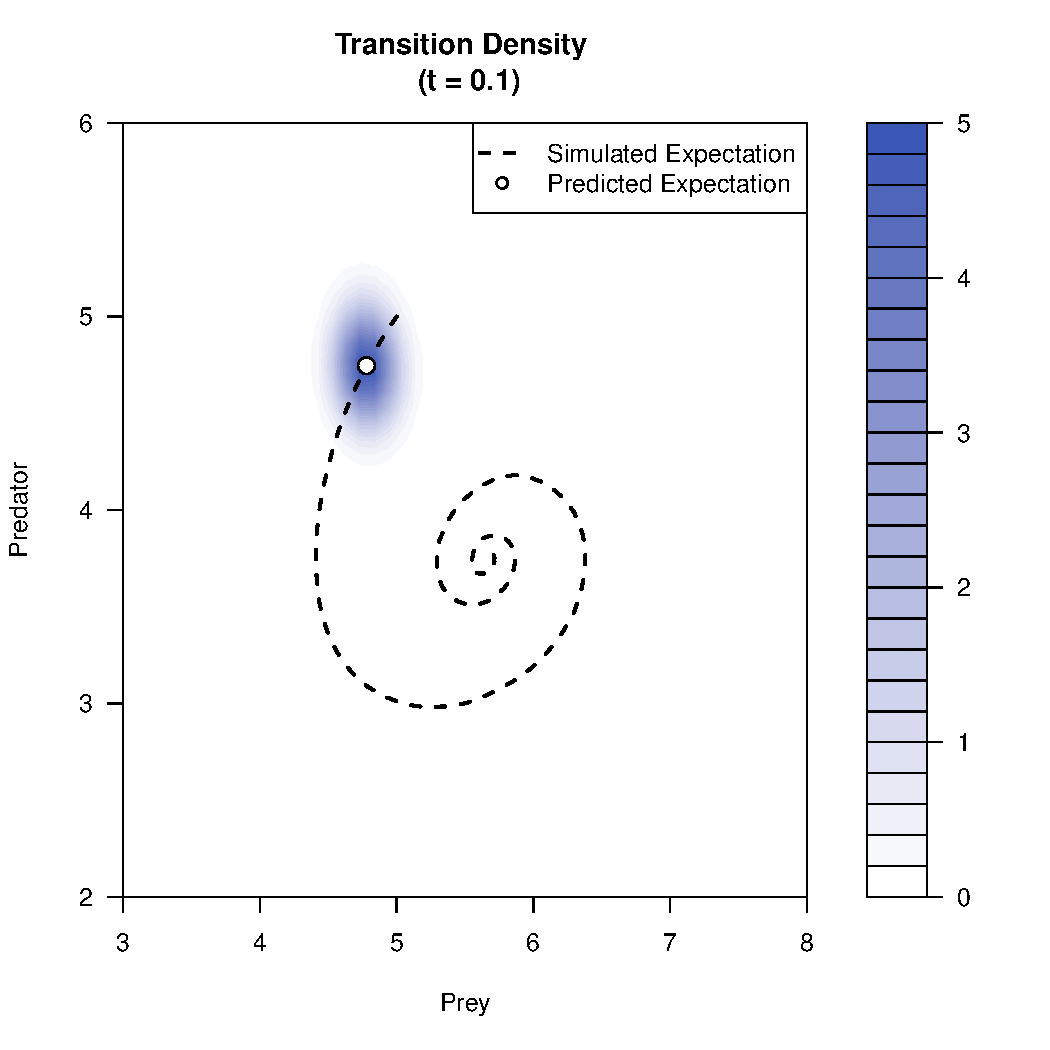
\includegraphics[width=4in,height=4in]{figure/GQD-coupledPlot-1} 

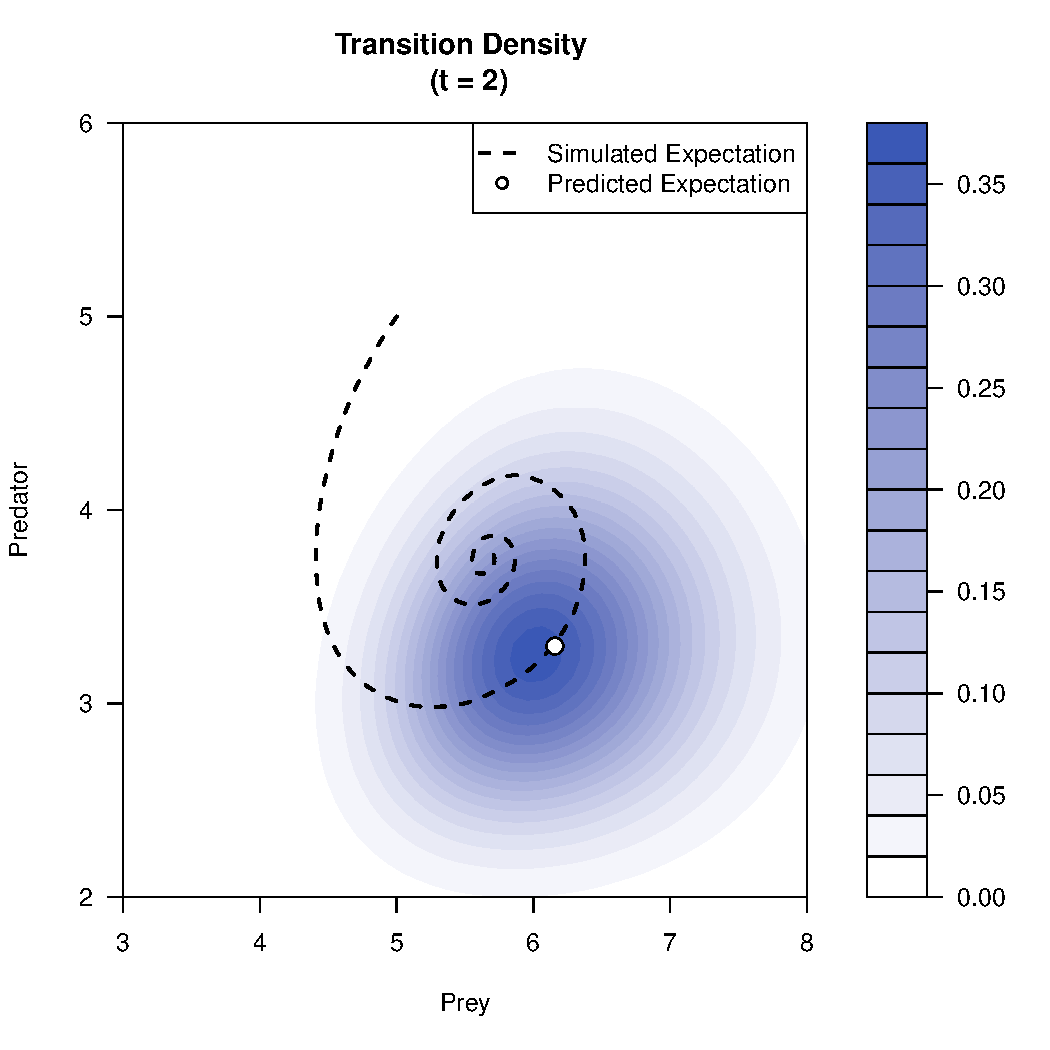
\includegraphics[width=4in,height=4in]{figure/GQD-coupledPlot-2} 

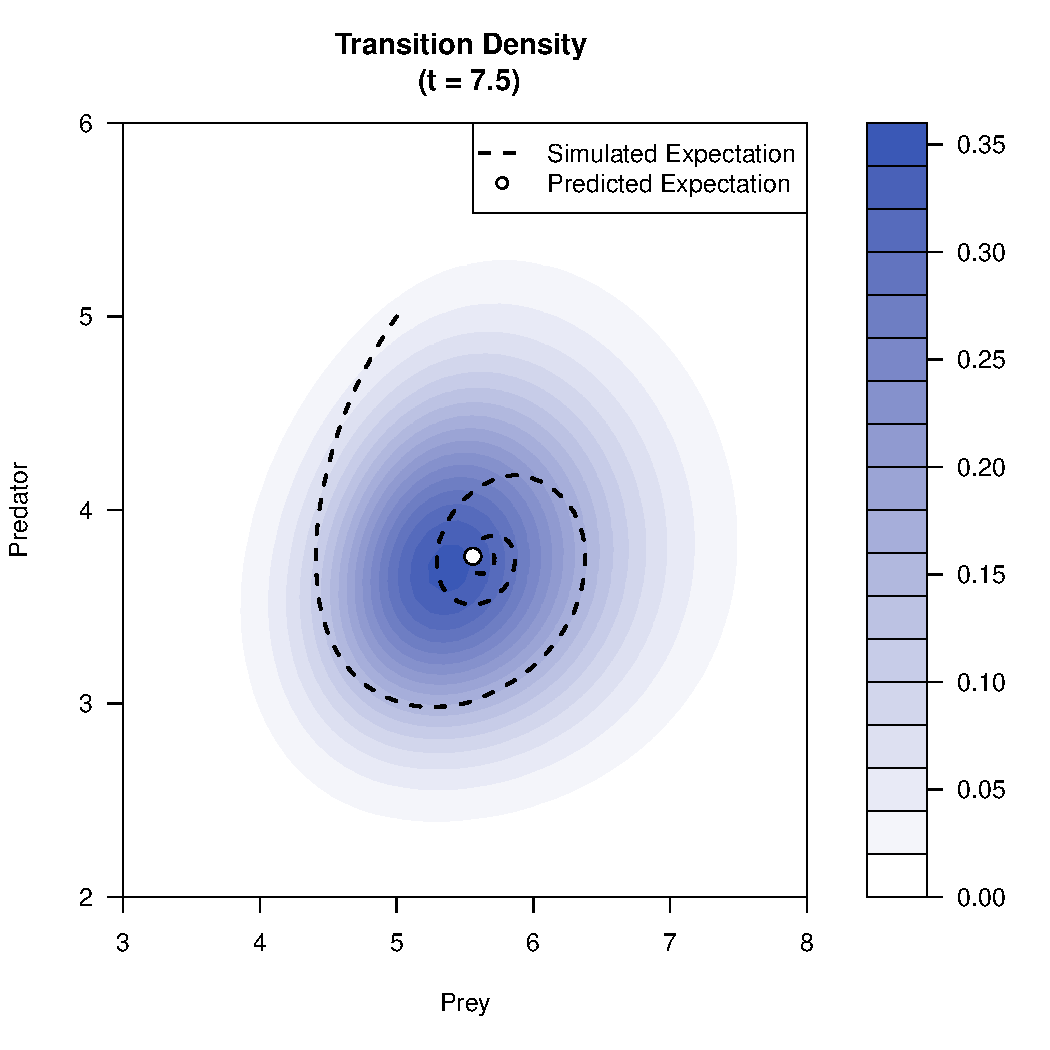
\includegraphics[width=4in,height=4in]{figure/GQD-coupledPlot-3} 

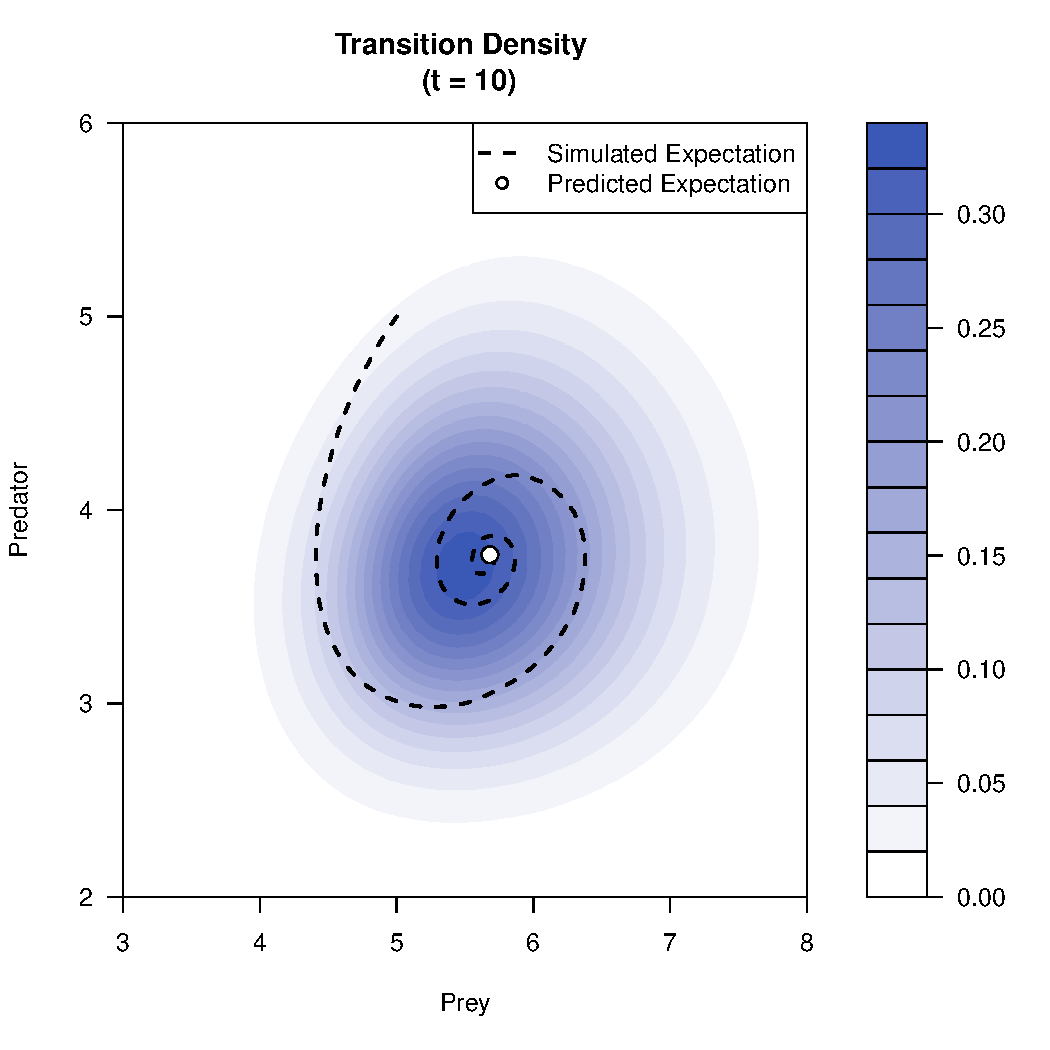
\includegraphics[width=4in,height=4in]{figure/GQD-coupledPlot-4} 

\end{knitrout}

\subsection{Inference on Diffusion Processes}
\begin{knitrout}
\definecolor{shadecolor}{rgb}{0.969, 0.969, 0.969}\color{fgcolor}\begin{kframe}
\begin{alltt}
\hlkwd{library}\hlstd{(}\hlstr{"DiffusionRgqd"}\hlstd{)}
\hlkwd{data}\hlstd{(SDEsim1)}
\hlkwd{attach}\hlstd{(SDEsim1)}
\end{alltt}


{\ttfamily\noindent\itshape\color{messagecolor}{\#\# The following object is masked \_by\_ .GlobalEnv:\\\#\# \\\#\#\ \ \ \  Xt}}

{\ttfamily\noindent\itshape\color{messagecolor}{\#\# The following object is masked from SDEsim3:\\\#\# \\\#\#\ \ \ \  time}}\begin{alltt}
\hlkwd{par}\hlstd{(}\hlkwc{mfrow}\hlstd{=}\hlkwd{c}\hlstd{(}\hlnum{1}\hlstd{,}\hlnum{1}\hlstd{))}
\hlstd{expr1}\hlkwb{=}\hlkwd{expression}\hlstd{(dX[t]}\hlopt{==}\hlnum{2}\hlopt{*}\hlstd{(}\hlnum{5}\hlopt{+}\hlnum{3}\hlopt{*}\hlkwd{sin}\hlstd{(}\hlnum{0.5}\hlopt{*}\hlstd{pi}\hlopt{*}\hlstd{t)}\hlopt{-}\hlstd{X[t])}\hlopt{*}\hlstd{dt}\hlopt{+}\hlnum{0.5}\hlopt{*}\hlkwd{sqrt}\hlstd{(X[t])}\hlopt{*}\hlstd{dW[t])}
\hlkwd{plot}\hlstd{(SDEsim1}\hlopt{$}\hlstd{Xt}\hlopt{~}\hlstd{SDEsim1}\hlopt{$}\hlstd{time,} \hlkwc{type} \hlstd{=} \hlstr{'l'}\hlstd{,} \hlkwc{col} \hlstd{=} \hlstr{'#222299'}\hlstd{,} \hlkwc{xlab} \hlstd{=} \hlstr{'Time (t)'}\hlstd{,} \hlkwc{ylab} \hlstd{=} \hlkwd{expression}\hlstd{(X[t]),} \hlkwc{main} \hlstd{= expr1)}
\end{alltt}
\end{kframe}
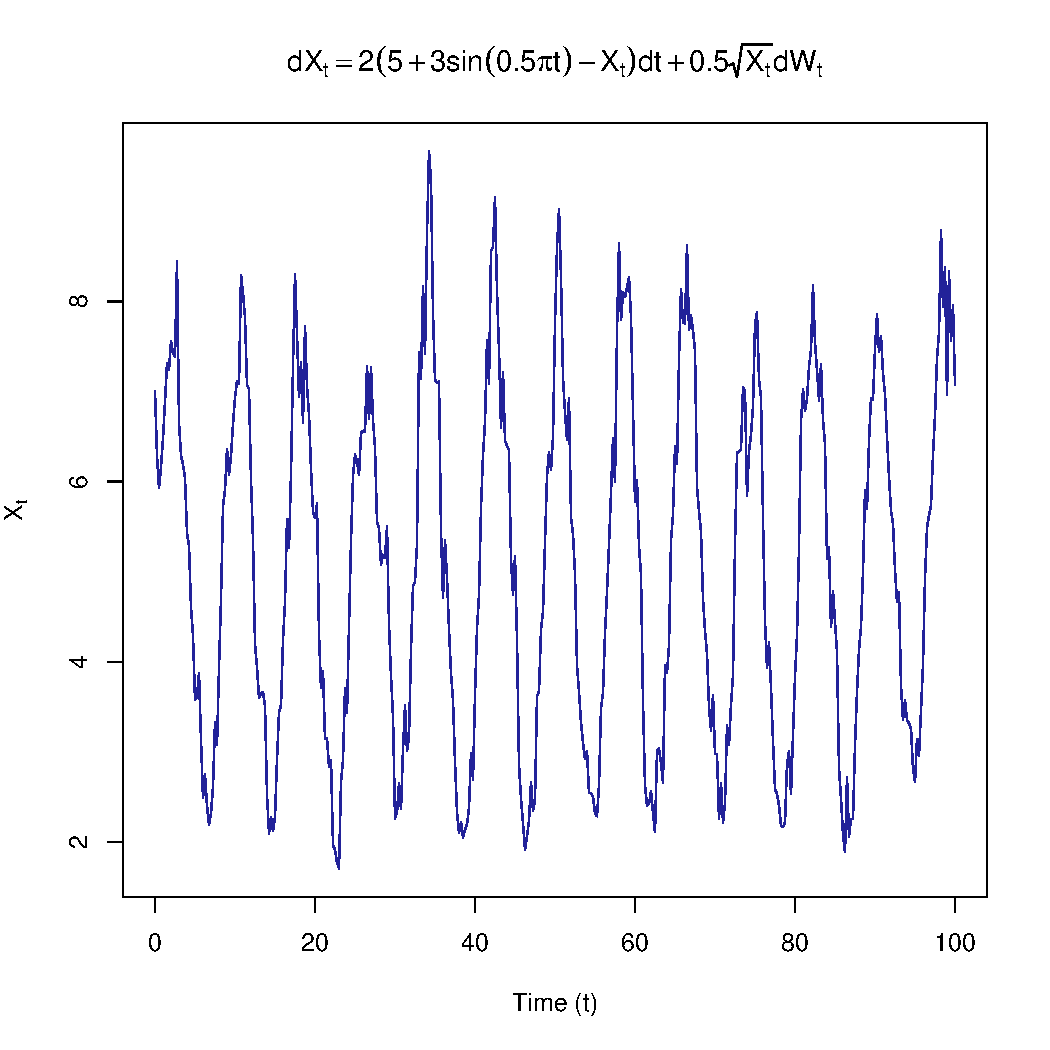
\includegraphics[width=4in]{figure/GQD-inference-1} 

\end{knitrout}

\begin{knitrout}
\definecolor{shadecolor}{rgb}{0.969, 0.969, 0.969}\color{fgcolor}\begin{kframe}
\begin{alltt}
\hlkwd{GQD.remove}\hlstd{()}

\hlstd{G0} \hlkwb{<-} \hlkwa{function}\hlstd{(}\hlkwc{t}\hlstd{)\{theta[}\hlnum{1}\hlstd{]}\hlopt{*}\hlstd{(theta[}\hlnum{2}\hlstd{]}\hlopt{+}\hlstd{theta[}\hlnum{3}\hlstd{]}\hlopt{*}\hlkwd{sin}\hlstd{(}\hlnum{0.25}\hlopt{*}\hlstd{pi}\hlopt{*}\hlstd{t))\}}
\hlstd{G1} \hlkwb{<-} \hlkwa{function}\hlstd{(}\hlkwc{t}\hlstd{)\{}\hlopt{-}\hlstd{theta[}\hlnum{1}\hlstd{]\}}
\hlstd{Q1} \hlkwb{<-} \hlkwa{function}\hlstd{(}\hlkwc{t}\hlstd{)\{theta[}\hlnum{4}\hlstd{]}\hlopt{*}\hlstd{theta[}\hlnum{4}\hlstd{]\}}

\hlstd{theta}   \hlkwb{<-} \hlkwd{c}\hlstd{(}\hlnum{1}\hlstd{,} \hlnum{10}\hlstd{,} \hlnum{1}\hlstd{,} \hlnum{1}\hlstd{)}               \hlcom{# Starting values for the chain}
\hlstd{sds}     \hlkwb{<-} \hlkwd{c}\hlstd{(}\hlnum{0.25}\hlstd{,} \hlnum{0.25}\hlstd{,} \hlnum{0.2}\hlstd{,} \hlnum{0.05}\hlstd{)}\hlopt{/}\hlnum{1.5} \hlcom{# Std devs for proposal distributions}
\hlstd{mesh}    \hlkwb{<-} \hlnum{10}                           \hlcom{# Number of mesh points}
\hlstd{updates} \hlkwb{<-} \hlnum{110000}                       \hlcom{# Perform 110000 updates}
\hlstd{burns}   \hlkwb{<-} \hlnum{10000}                        \hlcom{# Burn 10000 updates}

\hlcom{# Run the MCMC procedure for the model defined above:}
\hlstd{model_1} \hlkwb{<-} \hlkwd{GQD.mcmc}\hlstd{(SDEsim1}\hlopt{$}\hlstd{Xt, SDEsim1}\hlopt{$}\hlstd{time, mesh, theta, sds, updates, burns)}
\end{alltt}
\end{kframe}
\end{knitrout}

% TODO: Fix input

% <<GQD-RanOnRSeparately>>=
% _____________________ Drift Coefficients _______________________
% G0 : theta[1]*(theta[2]+theta[3]*sin(0.25*pi*t))                
% G1 : -theta[1]                                                  
% G2                                                              
% ___________________ Diffusion Coefficients _____________________
% Q0                                                              
% Q1 : theta[4]*theta[4]                                          
% Q2                                                              
% _____________________ Prior Distributions ______________________
                                                             
% d(theta):None.                                                  
% @

% TODO: Add the inference plot

The estimates are given by

\begin{knitrout}
\definecolor{shadecolor}{rgb}{0.969, 0.969, 0.969}\color{fgcolor}\begin{kframe}
\begin{alltt}
\hlkwd{GQD.estimates}\hlstd{(model_1,} \hlkwc{thin} \hlstd{=} \hlnum{100}\hlstd{,} \hlkwc{burns} \hlstd{=} \hlnum{10000}\hlstd{,} \hlkwc{corrmat} \hlstd{=} \hlnum{TRUE}\hlstd{)}
\end{alltt}
\end{kframe}
\end{knitrout}

% TODO: Fix the results
% <<GQD-estimatesResult>>=
%          Estimate lower_CI upper_CI
% theta[1]    2.026    1.820    2.256
% theta[2]    5.016    4.922    5.106
% theta[3]    2.915    2.787    3.050
% theta[4]    0.501    0.472    0.534

% $corrmat
%          theta[1] theta[2] theta[3] theta[4]
% theta[1]     1.00    -0.19    -0.36     0.38
% theta[2]    -0.19     1.00     0.35    -0.03
% theta[3]    -0.36     0.35     1.00    -0.13
% theta[4]     0.38    -0.03    -0.13     1.00
% @

% TODO: Add the trace plot

\section{pomp: statistical inference for partially-observed Markov processes}
\section{Robfilter}
\section{Sim.DiffProc Package - FitSDE}
\section{HPloglik}
\section{abctools}

\end{document}
